\documentclass{article}


% if you need to pass options to natbib, use, e.g.:
%     \PassOptionsToPackage{numbers, compress}{natbib}
% before loading neurips_2023

% for algorithm
\usepackage{algorithm}
\usepackage{algpseudocode}

% ready for submission
\usepackage[final]{neurips_2023}


% to compile a preprint version, e.g., for submission to arXiv, add add the
% [preprint] option:
%     \usepackage[preprint]{neurips_2023}


% to compile a camera-ready version, add the [final] option, e.g.:
%     \usepackage[final]{neurips_2023}


% to avoid loading the natbib package, add option nonatbib:
%    \usepackage[nonatbib]{neurips_2023}


\usepackage[utf8]{inputenc} % allow utf-8 input
\usepackage[T1]{fontenc}    % use 8-bit T1 fonts
\usepackage{hyperref}       % hyperlinks
\usepackage{url}            % simple URL typesetting
\usepackage{booktabs}       % professional-quality tables
\usepackage{amsfonts}       % blackboard math symbols
\usepackage{nicefrac}       % compact symbols for 1/2, etc.
\usepackage{microtype}      % microtypography
\usepackage{xcolor}         % colors
\usepackage{graphicx}       % allows images

\graphicspath{ {./images/} }


\title{Predicting Fluctuating Commodity Prices using Random Forests}


% The \author macro works with any number of authors. There are two commands
% used to separate the names and addresses of multiple authors: \And and \AND.
%
% Using \And between authors leaves it to LaTeX to determine where to break the
% lines. Using \AND forces a line break at that point. So, if LaTeX puts 3 of 4
% authors names on the first line, and the last on the second line, try using
% \AND instead of \And before the third author name.

\author{
  Bosli, Massinissa \\
  EC 503 Student\\
  Boston University\\
  Boston, MA 02215 \\
  \texttt{myb24@bu.edu} \\
  % examples of more authors
  \And
  Jamias, Austin \\
  EC 503 Student\\
  Boston University\\
  Boston, MA 02215 \\
  \texttt{ajamias@bu.edu} \\
  \AND
  Ehrlich, Ben \\
  EC 503 Student\\
  Boston University\\
  Boston, MA 02215 \\
  \texttt{behrlich@bu.edu} \\
  \And
  Bensadon, Moises \\
  EC 503 Student\\
  Boston University\\
  Boston, MA 02215 \\
  \texttt{moises@bu.edu} \\
  \And
  Yadav, Mayank \\
  EC 503 Student\\
  Boston University\\
  Boston, MA 02215 \\
  \texttt{mayanky@bu.edu} \\
}


\begin{document}


\maketitle


\begin{abstract}
In this paper, we present an analysis of a variety of methods using decision and regression trees to predict commodity prices. The aim of the study is to compare the different ways one can use trees to develop an accurate and efficient model for price prediction that can be applied for various commodities such as airline tickets, food prices, etc. We used a dataset of over 300,000 airline tickets to train decision trees \& random forests of various sizes. We found the random forest model performed the best out of the chosen models and was able to outperform a singular decision tree consistently on the test and validation data. The reasonable errors reported show that a random forest model has the potential to make accurate price predictions.
\end{abstract}


\section{Introduction}

With the abundance of data in today's day and age, there is an increasing amount of uncertainty about the data without the correct tools to interpret it. It can be difficult to predict the fluctuating prices of resources such as airline tickets without the right tools and information. There exists machine learning models that do just this through supervised learning. However, with categorical data the basic regression problem becomes ineffective. The decision tree is one solution that we examined because it provides support for categorical variables. Since there were many ways to implement a decision tree, we decided to test and compare the performances between a selection of chosen models. We searched for the model with the best test accuracy among the decision trees \& random forests. Although many Kaggle competition winners utilized boosting as their main method of training, we hypothesized that random forests would perform the best because current theories suggest that they reduce over-fitting in decision tree. 

Other papers exist of varying quality aimed at solving this problem, but many previous attempts have not solved the problem with low enough error, or were strictly theoretical and lacked empirical testing, or missed the right complexity for the problem of flight ticket price prediction. With this paper, we hope to approach the problem in a robust way, resulting in a procedure proven to work, which could be retrained on different regions, commodities, etc with minimal effort.


\section{Related Works}
\label{gen_inst}

\subsection{Decision Trees}

Widely used in a range of applications, Decision Trees became highly popular thanks to their simplicity and human-interpretability. When boosted, DT are provably robust against adversarial attacks \cite{Maksym}, and are highly efficient. They are understood widely interpreting categorical data, but also have uses with some loosening of constraints for mixed and numerical datasets. Instead of creating branches to increase purity, branches are created to minimize mean squared error and have seen provable and empirical success \cite{Luo}.

\subsection{Gradient Boosted Decision Trees (GBDT)}

Feng et al. discuss more in-depth the application of gradient boosted decision trees for multi-layer models used in many deep learning applications \cite{Feng}. Described in the paper, MLGBDT extends traditional gradient boosting methods by adding additional layers of decision trees, where each layer learns the residuals of the previous layer. Unlike AdaBoost, GBDT trains an ensemble of trees by feeding the residuals of the previous tree as labels to the next tree with the aim of learning all the residuals and summing to a more accurate prediction. Feng et al. introduce MLGBDT that train independent GBDTs on different subsets on the data then output a weighted average. While the paper is primarily focused on DL, it does a decent job at summarizing the development of uses of boosted decision trees (DT) in multiple applications, discussing uses in Marketing, Quantum Physics, and Data Science. 

\subsection{Random Forest Ensembles (RF)}

Random forests are an ensemble of tree predictors each trained with a random sampling from the feature set and training set. While there are arguably many ways to approach the growth of trees in the forest, the first researchers to propose them used them in a way similar to AdaBoost.  Due to the random nature of trees, the generalization of the ensemble tends to be greater than other methods. This resistance to over-fitting in a general sense is discussed in Kleinberg's 1996 paper \cite{Kleinberg}. Stochastic models' performance drop tends to be smaller than analogous learning models without the stochastic elements when given huge amounts of data, implying a type of resistance to over-fitting. Random forests have resulted in significant improvements in classification accuracy by growing an ensemble of trees and letting them vote for the most popular class.

\section{Proposed Methods}
\label{headings}

\subsection{Regression Tree}

The decision tree is a well-known algorithm that is relatively simple to comprehend. At its core, the algorithm comprises a series of decision stumps, which continue to divide the data using a basic splitting rule. Consider an input \(x\) with \(d\) features. Based on the root node's splitting rule, which is based on one of the \(d\) features, \(x\) is assigned to one of the two child nodes. These child nodes, in turn, have their own splitting rules that dictate the assignment of \(x\) to their child nodes. This recursive process continues until \(x\) reaches a node without child nodes or splitting rules, which is denoted as a leaf. This leaf node is assigned a label, which is used to predict the output of \(x\). Figure 1 illustrates this process.

\begin{figure}[h]
\caption{Visualization of Decision Tree construction}
\centering
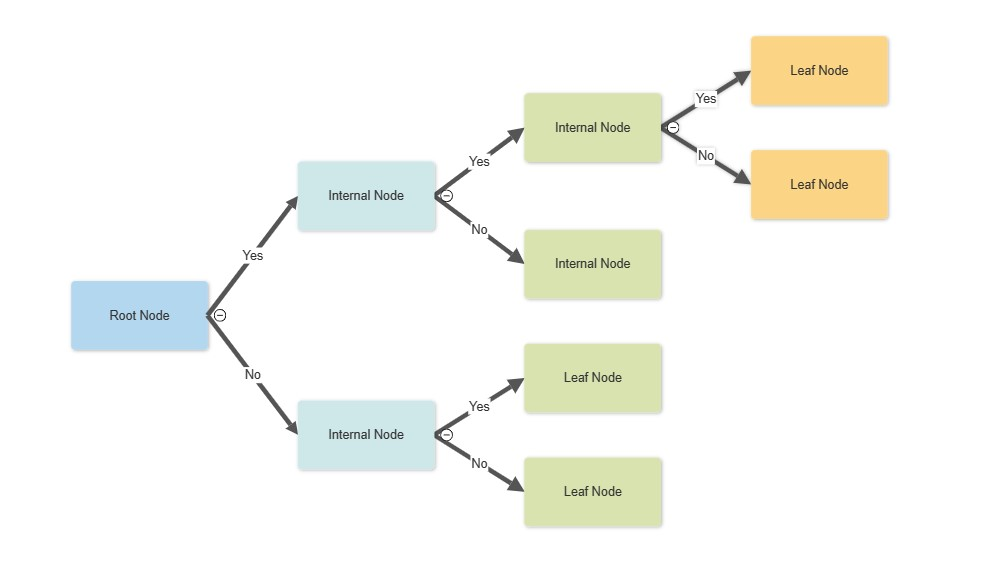
\includegraphics[width=0.85\textwidth]{Fig1}
\end{figure}

The construction of such a tree, also termed “growing," is performed utilizing a top-down “greedy” approach. Starting from the root node, splitting rules are decided and made on all of the training data, resulting in two child nodes, the recursive process repeats on each of the child nodes until no split is possible, or a set condition has been met. The “greediness” of this algorithm derives from the approach used to decide on a splitting rule. The splitting rule of the decision stump at each node is designed to reduce the uncertainty of the split. This is usually done by measuring the uncertainty of splitting on every unique value of every feature on the training data S. The whole procedure is summarized in Algorithm 1.

The measure of uncertainty of a split can be measured in a plethora of ways. In the case of classification, popular methods of measuring the uncertainty are the gini impurity and entropy. Gini impurity measures the degree or probability of miss-classification, while entropy measures the degree of disorder or randomness in a data set. Both measures of uncertainty are however incompatible with a regression problem, which is the focus here. Thus other methods are employed to measure the uncertainty, such as the reduction in the mean squared error (MSE reduction). The mean squared error of each node is a sum of the squared distance between all the data in the node and their labels multiplied by the weight of each sample

\begin{equation}
f(n) = \sum_{i=1}^m{P(i)(\hat{y}_{n} - y_{i})^2}
\end{equation}

The probability of each node occurring is calculated to be the sum of the weights of the samples in the node

\begin{equation}
W_{n} = \sum_{i=1}^m{P(i)}
\end{equation}

The MSE reduction is just the difference between the MSE of the parent node \(p\) and its two child nodes \(a\) and \(b\) all proportional to their probabilities. The resulting objective function is the maximization of the MSE reduction for each split \(g\)

\begin{equation}
\arg \max_{g}   W_{n_{p}}f(n_{p}) - W_{n_{a}}*f(n_{a}) - W_{n_{b}}*f(n_{b})
\end{equation}

As shown in Algorithm 1, this maximization of the MSE reduction is computed by computing the MSE reduction on all possible splits for each node. It is worth noting that in the context of real-world data, features of the data are rarely just continuous or categorical, but usually a mixture of both. This poses a potential challenge in deciding a splitting rule as a splitting rule for continuous data is not usually compatible with categorical data. The splitting rule must then change depending on the type of data each feature presents. In the case of continuous data, a decision stump splits according to a specified value to which samples are split whether their feature is above or below the value. Categorical data, on the other hand, a one-vs-all method is utilized.

Traditionally, a decision or regression tree will stop splitting the nodes when under certain conditions. The application of these predetermined conditions is called pre-pruning; its aim is to reduce the over-fitting of the tree. In our implementation of a regression, no conditions were applied. The availability of such a large data set reduced the chance of over-fitting.

\begin{algorithm}[ht]
\caption{Top-Down Greedy Decision Tree Algorithm (CART)}
\begin{algorithmic}[1]
\State \textbf{Input:} Sample $S$ of $m$ points with $d$ features
\State \textbf{Initialization:} Root Node contains all training data $m$
\Procedure{DecisionTree}{$node$}
    \If{node meets termination conditions}
        \State set $node \to$ leaf with a label and end
    \EndIf
    \ForAll{features $d$}
        \ForAll{$j$ unique values in features $d$}
            \State split data on feature $j$
            \State calculate uncertainty
            \State find $j$ with min uncertainty
        \EndFor
    \EndFor
    \State split nodes of features $d$ by value $j$
    \State repeat for each child node
\EndProcedure
\end{algorithmic}
\end{algorithm}

\subsection{Ensemble Methods:}

The tendency of decision trees, including regression trees, to over-fit is one of the reasons the algorithm is usually used in ensemble. A variety of ensemble methods exist, but Breiman’s application of Random Forests and his conjecture that AdaBoost is a random forest made this ensemble method extremely appealing \cite{Breiman}.

\subsubsection{Random Forests}

Our implementation of a Random Forrest is very similar to Breiman’s approach. Multiple decision trees are built using the top-down “greedy” algorithm. A different sub-sample of the training data was taken with replacement and used to train each tree. Breiman also used a set of random features k for each tree in the forest. Our approach neglected to add this layer of stochasticity as we found that it only increased the validation error. Once each decision tree is constructed, the prediction of the forest is, in the case of regression, the mean of the predictions of all the trees. The procedure for this implementation is shown in Algorithm 2.

The number of trees, denoted T, is the only hyper-parameter utilized in our implementation of a random forest. Breiman theorizes that the generalization error is upper-bounded as such as T approaches infinity \cite{Breiman}.

It is important to note that although using a maximum number of trees seems like a reasonable method to continue, the construction of each tree takes $O(n m \cdot{} \log(n))$ time. So growing a random forest will take $O(T \cdot{} n m \cdot{} \log(n))$. As a result, the optimal T is one where the generalization error ceases to decrease significantly with respect to the time complexity. This optimal T will be found using validation data.


\begin{algorithm}[ht]
\caption{Growing a Random Forest}
\begin{algorithmic}[1]
\State \textbf{Input:} Sample $S$ of $m$ points with $d$ features
\For{$I = 1, 2, 3, \dots, T$} \Comment{$T$ is the number of trees (hyperparameter)}
    \State Generate a random variable $\theta$ by sampling $S$ with replacement
    \State Choose $k$ random features (either $k = \sqrt{d}$ or $k = \log{d}$)
    \State Grow a decision tree (Top-Down Greedy Algorithm) on $\theta$ with $K$ features
\EndFor
\State \textbf{Output:} Predictions are the mean or mode of all decision tree predictions
\end{algorithmic}
\end{algorithm}




\section{Results}
\label{others}

All models in our experimentation were trained using a dataset of over 300,000 data points from Kaggle \cite{kaggle}. This data was taken from the website “Ease My Trip” over the course of 50 days: February 11th to March 31st, 2022. Each data point consisted of ten features and the label which was the price of the ticket. A breakdown of the dataset can be found in Table 1 \& Table 2.

\begin{table}[ht]
  \caption{Data set Features}
  \label{sample-table}
  \centering
  \begin{tabular}{lll}
    \toprule
    Feature     & Data Type     & \# of classes \\
    \midrule
    Airline     & Categorical   & 6     \\
    Flight      & N/A   & N/A     \\
    Source City & Categorical   & 6     \\
    Departure Time  & Categorical   & 6     \\
    Stops       & Categorical   & 3     \\
    Arrival Time    & Categorical   & 6     \\
    Destination City    & Categorical   & 6     \\
    Class   & Categorical   & 2     \\
    Duration    & Continuous   & N/A    \\
    Days Left   & Continuous   & N/A     \\
    \midrule
    Price       & Continuous   & N/A     \\

    \bottomrule
  \end{tabular}
\end{table}

\begin{table}[h]
  \caption{Data set Partitions}
  \label{sample-table}
  \centering
  \begin{tabular}{lll}
    \toprule
    Partition       & \# of Points \\
    \midrule
    Training        & 10000 \\
    Validation      & 50000 \\
    Test            & 240153 \\
    \bottomrule
  \end{tabular}
\end{table}

To get a complete picture of the data set, a histogram of the data was taken (Figure 2). The results show that the prices of the tickets are centered around two means, with the majority of the prices around 100 dollars.

\begin{figure}[ht]
\caption{Histogram of Prices in Data set}
\centering
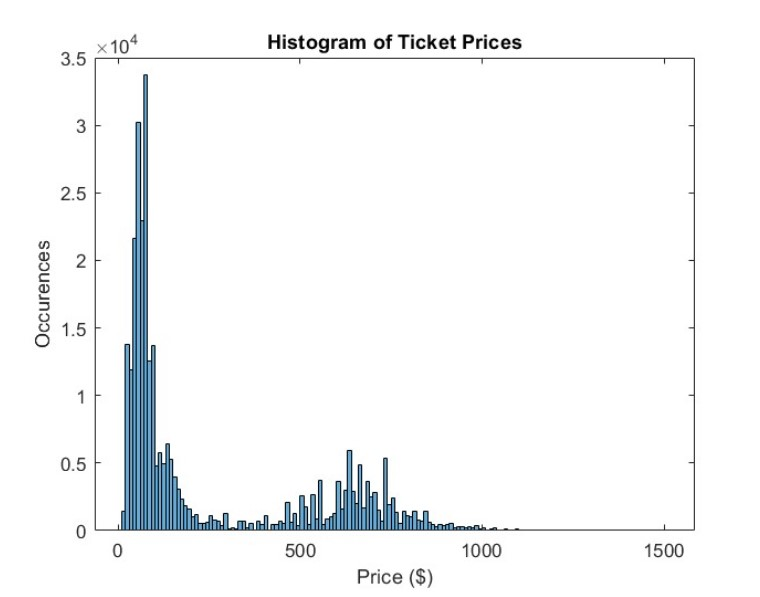
\includegraphics[width=0.7\textwidth]{Fig2}
\end{figure}

\subsection{Baseline Error}

In these regression problems, the error is measured using the mean squared error (MSE). Measuring the error in such a way is less intuitive than measuring the percent accuracy or error of classification problems. For example, a root mean squared error (RMSE) of 5 tells us that, on average, the prediction price is about 5 dollars off the true price. This measure results in different conclusions depending on the data. If the prices range in the hundreds of dollars then an average error of 5 is pretty reasonable. The opposite would be true if the price range was around 5 dollars.

We combat this confusion in two ways. First, we design the most basic decision tree and compare its RMSE against the models of our design. The most basic decision tree consists of a single node with a prediction of just the mean of all the data points. Such a predictor returns an RMSE of 276.84 on the test set. Another method to show the accuracy of the predictors is to graph the percent error of the predictions, which allows for a better understanding of how far off the data our predictors are.

\subsection{Regression Tree Results}

The construction of the singular regression tree was completed using a recursive structure in MATLAB. Each structure would correspond to a node and would call two child nodes as two of its elements. The recursive call of a function builds the tree according to the top-down standard CART algorithm discussed. The tree was constructed with the only stopping condition being if the MSE reduction was less than or equal to zero. At the completion of tree construction, a visual representation of the tree was produced using MATLAB's directed graphs (Figure 3). The abundance of splits and nodes indicates that this tree is in danger of over-fitting the test set.

\begin{figure}[ht]
\caption{Visualization of the Regression Tree}
\centering
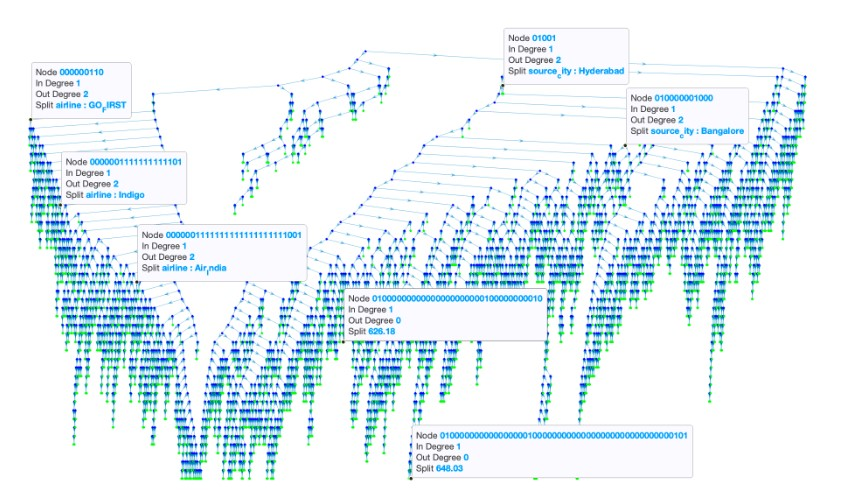
\includegraphics[width=0.85\textwidth]{Fig3}
\end{figure}

The reported training RMSE of the regression tree was significantly lower than the test RMSE. This confirms that the tree is over-fitting the data, but that was to be expected from a tree with no pre-pruning. Compared to the most simple regression tree, the new model performed extremely well.

\begin{table}[ht]
  \caption{Regression Tree Results}
  \label{sample-table}
  \centering
  \begin{tabular}{lll}
    \toprule
    Model     & RMSE \\
    \midrule
    Single Node Test RMSE   &  276.84     \\
    Training RMSE       & 55.74       \\
    Test RMSE           & 70.27      \\

    \bottomrule
  \end{tabular}
\end{table}

A histogram of the data gives a better understanding of how far off the predictions were from their corresponding true values. According to Figure 4, the vast majority of the data was only about 10 percent off the true value.

\begin{figure}[ht]
\caption{Histogram of \% Difference (Regression Tree)}
\centering
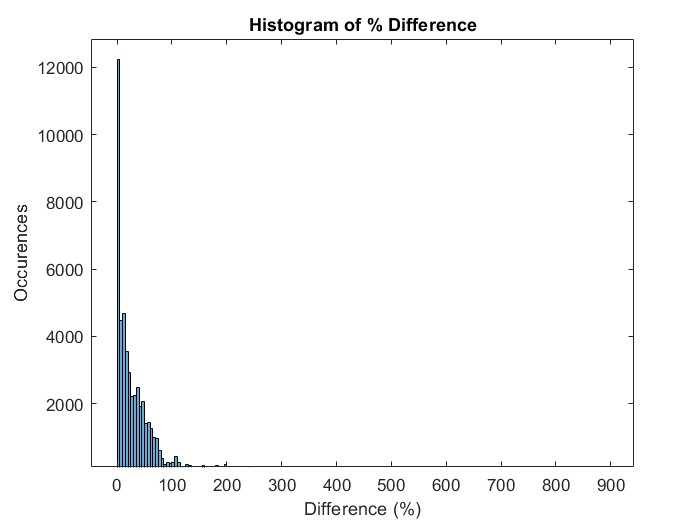
\includegraphics[width=0.7\textwidth]{Fig4}
\end{figure}

\subsection{Random Forest Results}

The random forest was implemented as Algorithm 2 described. To find an optimal T, validation was run on a set of random forests with increasing T from 20 to 70. Breiman states that the upper bound on the test error decreases with an increase in T, so running this validation serves two purposes: confirmation of the theory, and the measure of the cost of computation \cite{Breiman}. The larger T becomes, the higher the computational complexity of the algorithm. It is, for this reason, massive amounts of trees (on the order of hundreds or thousands) cannot be used.

\begin{figure}[h]
\caption{Validation MSE of RF on increasing T}
\centering
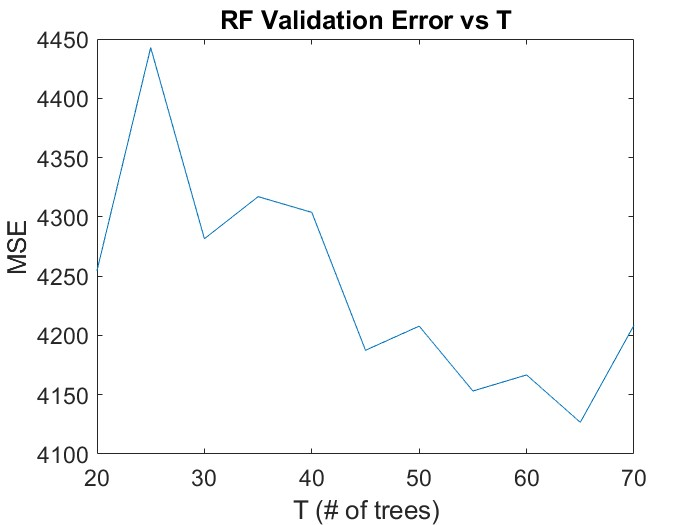
\includegraphics[width=0.85\textwidth]{Fig5}
\end{figure}

The data does confirm that the error does decrease with an increase in T. Long computational times prevented us from running validation sets on random forests larger than 70, however, the decrease in the MSE does seem to stochastically slow in the range of 60 to 70 trees, which resulted in a decision to use T = 65.

The resulting training and test error of the random forest displayed the generalization power of Random forests very well. The test error of the random forest was significantly lower than that of the singular regression tree. However, it is worth noting that the training error did significantly increase compared to the singular decision tree.

\begin{table}[ht]
  \caption{Random Forest Results}
  \label{sample-table}
  \centering
  \begin{tabular}{lll}
    \toprule
    Model     & RMSE \\
    \midrule
    Training RMSE       & 62.79       \\
    Test RMSE           & 64.24      \\
    \bottomrule
  \end{tabular}
\end{table}

A histogram of the percent difference once again shows that the majority of the predictions were only about 10 percent off their true value, however, the distribution of the percent error is more distributed than the resulting distribution of the singular decision tree.

\begin{figure}[h]
\caption{Histogram of \% Difference (Random Forest)}
\centering
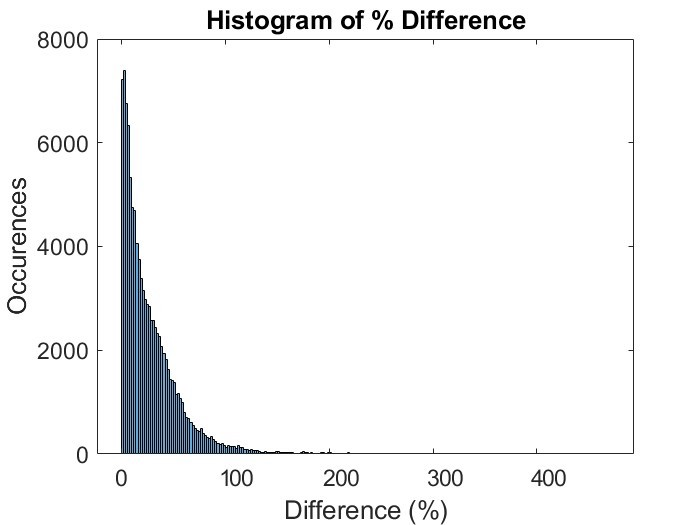
\includegraphics[width=0.7\textwidth]{Fig6}
\end{figure}


\section{Conclusion}

In this report, we presented an approach to using decision tree based models to predict airline ticket prices. Our project successfully demonstrated the potential of using a random forest algorithm for predicting future flight prices with a reasonable degree of accuracy. Our model achieved an RMSE of 62.7876 on the training set and 64.2394 on the test set, outperforming a single decision tree model, which exhibited over-fitting. This result validates the effectiveness of ensemble methods like random forests in mitigating over-fitting and improving generalization.

Another key factor we were exploring was the ability of random forests to generalize well to machine learning problems without a large amount of training data. Although our dataset consisted of about three hundred thousand data points, through repeated trials we realized we only needed ten thousand data points in our training set to optimize our test error. The test error of the singular decision tree was found to be higher than that of the random forest, while the training error of the same singular tree was reportedly lower than that of the random forest. This is an indication of over-fitting on the part of the singular decision tree. Utilizing the random forest decreased the variance of the model but increased the bias.

\subsection{Future Exploration}

Although our solution of using random forests worked well, there are numerous other ensemble methods we considered. Some of these including but not limited to:

\subsubsection{Gradient Boosting}

Even though the test error we reported was generally good, other ensemble methods may provide better results. One ensemble method that we might have implemented is Gradient Boosting, which is often used with regression trees. Furthermore, the use of multi-layered gradient boosting trees, proposed by Ji Feng, Yang Yu and Zhi-Hua Zhou, mimic the key feature of deep neural networks: multi-layered distributed representation \cite{Feng}. Such a method might be able to better distinguish patterns in the data over time, leading to more accurate results.

\subsubsection{Probabilistic Regression Trees}

A limitation of traditional regression trees is their inability to perfectly fit smooth continuous data. Sami Alkhoury et al. propose probabilistic regression trees to address the issue by introducing a probabilistic framework to tree-based models, potentially leading to improved predictions \cite{Alkhoury}. Applying this method to our project could further reduce the RMSE of the predictions and provide more accurate predictions for future flight prices. Additionally, this approach offers better interpretability by providing probabilistic estimates for each prediction, which could be valuable for decision-makers in the airline industry. Future work could explore the use of probabilistic regression trees in conjunction with other advanced machine-learning techniques to further enhance our flight price prediction model.

\subsection{Applications}

The accurate prediction of future flight prices has numerous practical applications and uses in the airline industry and for consumers alike. For airlines, understanding the factors affecting flight prices and anticipating price fluctuations can inform dynamic pricing strategies, helping companies optimize revenue management. With better predictions, airlines can make data-driven decisions on seat pricing, adjusting prices in response to demand, seasonality, or other market factors.

For travelers, a flight price prediction model can be a valuable tool in planning trips and budgeting for expenses. By providing insights into when flight prices are likely to rise or fall, the model can help consumers make informed decisions about when to book their flights, potentially leading to cost savings. Furthermore, travel agencies and online travel platforms can utilize the model to offer personalized flight recommendations, catering to individual preferences and budgets. Integrating the model into their services could provide a competitive advantage and enhance the user experience by helping customers find the best deals on flights.

In summary, an accurate flight price prediction model has wide-ranging applications across the airline industry and for consumers. From optimizing revenue management for airlines to aiding travelers in finding the best deals, the potential uses of such a model are vast and can contribute to more efficient and cost-effective travel experiences for all parties involved.

\subsection{Acknowledgments}

Special thanks to Professor Orabona for an informative and eye-opening semester.

\pagebreak

\bibliographystyle{plain}
\bibliography{citations/Maksym,citations/Luo,citations/Feng,citations/Kleinber,citations/Breiman,citations/kaggle,citations/Alkhoury}



%%%%%%%%%%%%%%%%%%%%%%%%%%%%%%%%%%%%%%%%%%%%%%%%%%%%%%%%%%%%


\end{document}